%# -*- coding: utf-8-unix -*-
%%==================================================
%% chapter02.tex for SJTU Bachelor Thesis
%%==================================================

\chapter{技术背景}
\label{chap:RL}

\section{系统虚拟化简介}
在计算机科学中,许多问题都可以通过增加或减少一个抽象层解决。在不同的场景下添加不同的抽象层,得到的结果大不相同。虚拟化技术即为一个抽象层。如果将该抽象层置于CPU,则会产生进程的概念,为系统中所有的任务抽象出可以独占的CPU,从而使得物理CPU的性能得到充分的利用。如果将该抽象层置于物理内存之上,则产生虚拟内存的概念,进程获得了一个连续的广阔的虚拟地址空间,虽然物理内存不一定是连续的。如果抽象出一个ISA(Instruction set architecture,指令集架构),即一个计算机运行的硬件环境,则产生了系统虚拟化(system virtualization)的概念。通过设计一个VMM(Virtual machine monitor, 虚拟机监控器),即可将客户机操作系统(Guest Operating System, Guest OS)运行在虚拟的硬件之上。系统虚拟化带来了诸多的好处,例如良好的封装性、硬件无关性\cite{sysv},这使得虚拟机可以在任何时候停止执行,通过快照在任何时间恢复先前的执行,这方便了虚拟机的热迁移,使得数据中心做到负载均衡。本文正是利用了这一优点。

历史上的虚拟化技术由纯软件虚拟化渐渐转向硬件辅助的虚拟化。早期的虚拟机监控器采用二进制翻译技术,是完全基于软件的虚拟化。由于软件模拟硬件行为的复杂性,纯软件的虚拟机监控器工程量巨大,代码复杂,同时性能相比于硬件环境有明显下降。之后学术界提出了半虚拟化(Para-Virtualization)技术来弥补纯软件虚拟化方式的不足。其想法是通过修改客户机操作系统,使得客户机明确知晓自己处在虚拟化环境中,与虚拟机管理器相互配合,避免了体系结构造成的虚拟化漏洞。最具有代表性的基于半虚拟化的虚拟机监控器就是Xen\cite{artofxen},客户机操作系统调用Xen提供的hypercall(虚拟化调用)配合VMM完成虚拟化功能。但是,由于Windows等闭源操作系统的存在,半虚拟化的可应用范围依然受限。现如今,基于硬件辅助的虚拟化大行其道,Intel推出的VT-x(Virtualization Technology for x86 processors)技术\cite{intelv}和AMD推出的SVM(Secure Virtual Machine Architecture)技术\cite{amdv}在现有的CPU指令集架构上增加了专用于虚拟化的指令,例如Intel的VMX指令\cite{intelSDM}。x86架构的处理器有两种运行模式,root mode(根模式)和non-root mode(非根模式),客户机运行在非根模式,当客户机需要执行特权指令时,触发VMexit,CPU运行模式由非根模式转换为根模式,通过trap-and-emulate(陷入并模拟)方式模拟客户机的特权指令。硬件辅助的虚拟化的优势在于,免去了对客户机的修改,由于客户机指令可以直接运行在宿主机的CPU上,又使得CPU虚拟化的代价大大减小。

对于内存虚拟化,传统的方式是为每一个客户机进程维护一个影子页表(SPT,shadow page table),将客户机进程的页表(GPT,guest page table)添加上由GPA(guest physical address,客户机物理地址)到HPA(host physical address,宿主机物理地址)的映射,于是SPT可以将GVA(guest virtual address,客户机虚拟地址)映射到HPA。然而当客户机进程数量较大时,影子页表维护和保存的开销将会十分可观。同时,由于客户机修改自己的页表(GPT)时SPT也要进行相应的修改,VMM将GPT所占的内存标记为写保护(write protected),当客户机修改GPT时会引起VMexit,退出到VMM中由VMM完成对SPT的维护。这对于memory intensive(内存密集)型任务是一种灾难,会引起大量的VMexit,严重影响其性能。Intel提出了EPT(Extended Page Table),使用硬件维护GPA到HPA的映射,用硬件替代了软件。如图\ref{fig:EPT}所示,客户机依然使用自己的CR3指针进行地址翻译,将GVA翻译为GPA,而虚拟机监控器为每一个客户机维护一张扩展页表,EPT base pointer(扩展页表基指针)指向扩展页表(EPT),将GPA通过硬件翻译为HPA。于是在客户机修改自身的GPT(guest page table)时无需引起VMexit,从而提高了性能。硬件上也有类似于传统页表TLB(translation look aside buffer)的应用于EPT的页表,缓存了EPTE(Extended Page Table Entry,扩展页表表项),加快了由GPA到HPA的翻译。使用本文所使用的巨型虚拟机即利用了这一硬件扩展,实现了内存的高效虚拟化。至于I/O虚拟化和中断虚拟化,则不在本文的讨论范围内。

\begin{figure}[!htp]
  \centering
  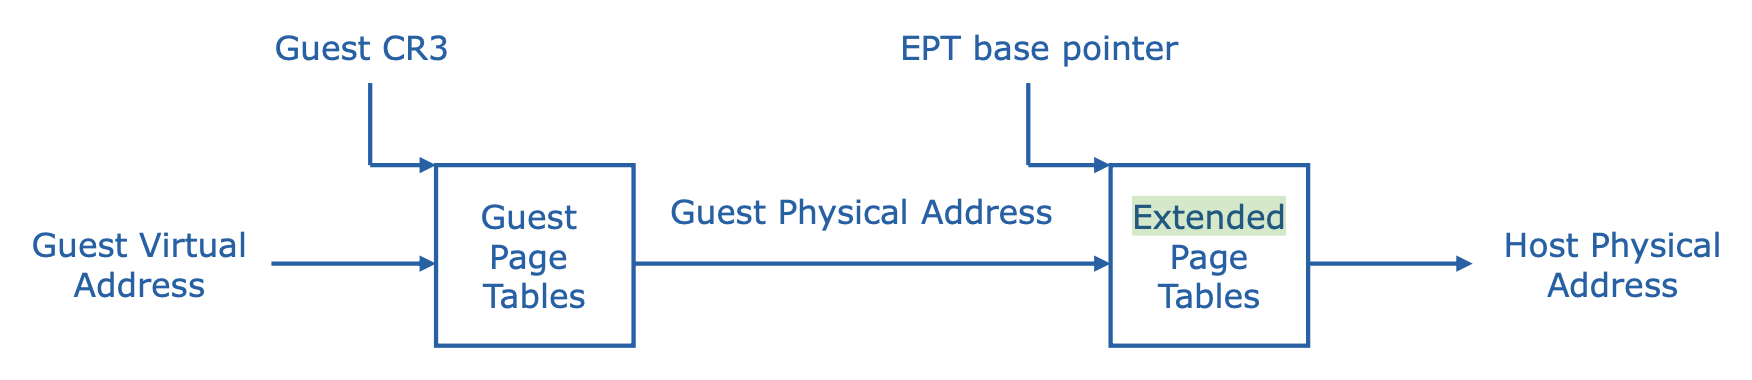
\includegraphics[width=15cm]{ept.png}
  \bicaption[扩展页表结构]
    {扩展页表(EPT)结构\cite{highperf}}
    {Structure of Extended Page Table}
  \label{fig:EPT}
\end{figure}

根据虚拟机监控器的软件架构,VMM又可分为Type-\uppercase\expandafter{\romannumeral1}型和Type-\uppercase\expandafter{\romannumeral2}型。Type-\uppercase\expandafter{\romannumeral1}型又称为Hypervisor型,该类型虚拟机监控器直接运行在裸金属上,直接负责虚拟机的创建、调度、运行、电源管理等,是一个完备的操作系统,所以需要编写大量驱动,工程量较大,但也具有更好的性能。而Type-\uppercase\expandafter{\romannumeral2}型虚拟机监控器运行在宿主机操作系统上,仅仅具有虚拟化的功能,而其他的功能由宿主机操作系统实现。还有混合型虚拟机监控器,它同样运行在裸金属上,但是将设备驱动、设备模型的控制权交由一个特权虚拟机。Xen属于混合性虚拟机,它将操作系统应当实现的功能交由domain 0这一特权操作系统完成。然而,Type-\uppercase\expandafter{\romannumeral1}型和混合型虚拟机需要修改客户机操作系统,依赖于客户机操作系统中的特定驱动,这对闭源操作系统而言是不现实的,同时减小了虚拟化的灵活性,故没有得到大范围应用。而开源虚拟机监控器QEMU-KVM属于Type-\uppercase\expandafter{\romannumeral1}型,KVM\cite{KVM}是Linux内核中的内核模块,而QEMU\cite{QEMU}是运行于用户态的宿主机应用程序,主要处理客户机的I/O请求,将KVM作为其虚拟化加速器,KVM利用x86处理器的VT-x、EPT等硬件辅助虚拟化功能获得了更优的虚拟机执行效率,而无需修改客户机操作系统,故得到了广泛的应用。下一节中的巨型虚拟机即通过修改QEMU-KVM这一开源虚拟机监控器得以实现。

\section{巨型虚拟机架构简述}
巨型虚拟机属于分布式虚拟机,即把一个分布式系统作为运行的物理基础,对上层提供统一的操作系统接口。其主要目的是为了资源聚合,即将分布式系统中的多个普通单机聚合起来,形成一个纵向扩展的虚拟机。举例而言,普通计算机的CPU核心数目一般在50以内,而更多CPU核心数目的机器则会非常昂贵\footnote{36个CPU核心是服务器较为典型的配置。详见 https://www.quora.com/What-are-the-specs-of-a-typical-modern-server}。有了巨型虚拟机,我们可以将多个普通且廉价的物理机聚合起来,启动一个拥有海量资源的虚拟机,例如将5个配备36个CPU的服务器进行资源聚集,我们可以得到一个拥有180个虚拟CPU的客户机,这是单个物理机很难达到的配置。
\begin{figure}[!htp]
  \centering
  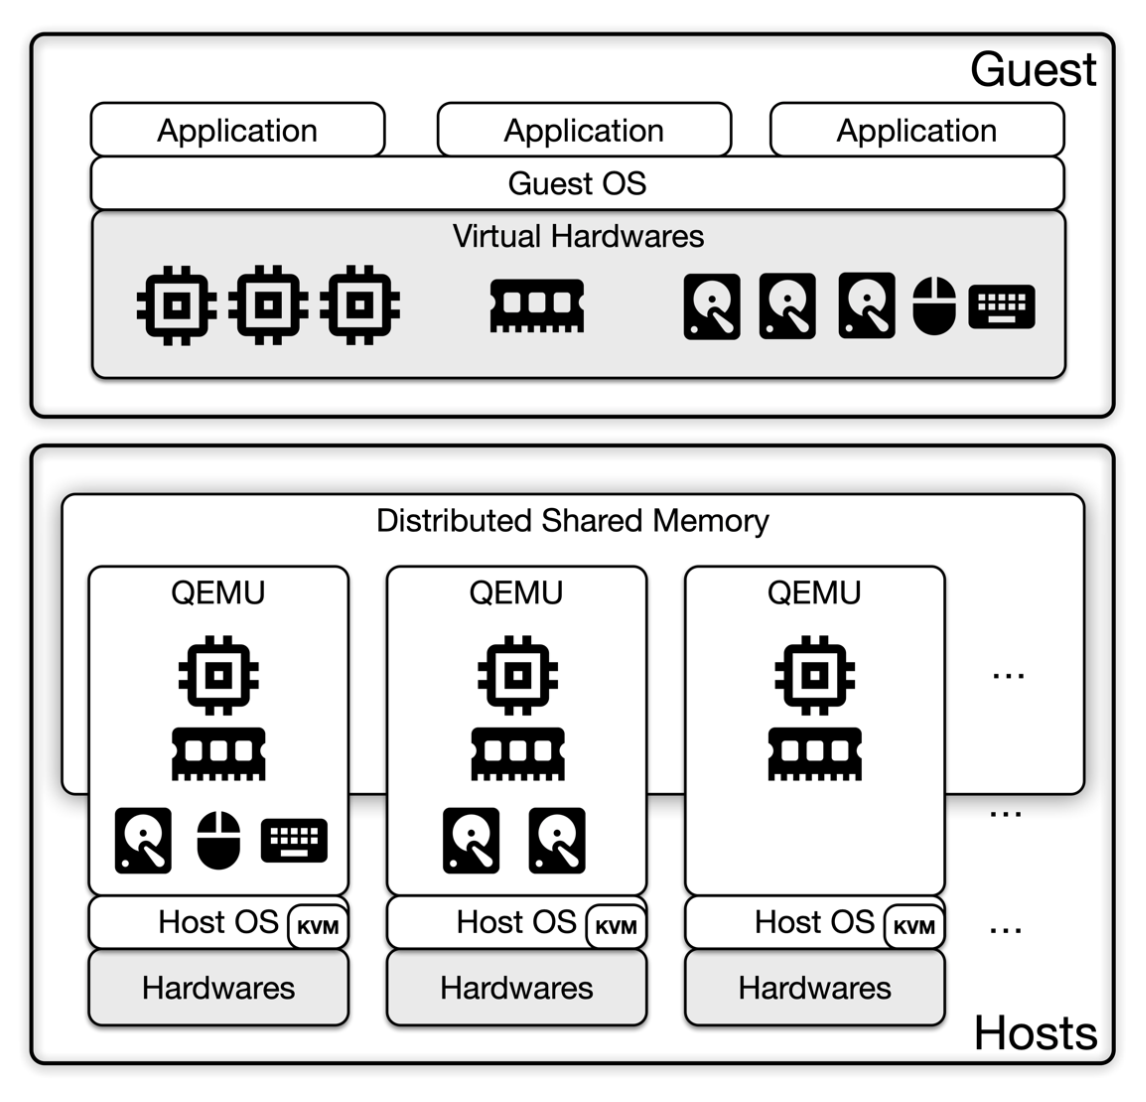
\includegraphics[width=10cm]{giantvm.png}
  \bicaption[巨型虚拟机架构]
    {巨型虚拟机架构\cite{giantvm}}
    {Architecture of GiantVM}
  \label{fig:SRR}
\end{figure}
巨型虚拟机基于QEMU-KVM这一Type-\uppercase\expandafter{\romannumeral2}型虚拟机监控器,将QEMU-KVM的功能扩展为分布式虚拟机。其实现主要分为三个部分,这与系统虚拟化常见的三个需要完成的部分相同:CPU虚拟化,内存虚拟化,I/O虚拟化。巨型虚拟机的架构如图 \ref{fig:SRR}所示。支持巨型虚拟机运行的基础设施是多个物理机组成的集群,在集群的每个节点上,都运行着一个巨型虚拟机的QEMU实例。每个实例都拥有整个集群的资源,但是属于本机的资源标记为local(本地资源),而集群中其他节点的资源标记为remote(远程资源)。当本地虚拟机实例对远程资源发起请求的时候,路由模块会找到所访问资源的真实位置,将资源请求转发到真正拥有该资源的节点上。而内存资源是一个例外:所有的虚拟机的QEMU实例拥有全部的内存资源,由DSM(distributed shared memory)进行提供。完成分布式虚拟化的三个主要功能模块有:
\begin{description}
    \item[分布式vCPU] 巨型虚拟机添加了新的QEMU参数,将一部分本地运行的vCPU标记为local vCPU,而其他未标记的vCPU则是remote vCPU。QEMU为所有的vCPU创建APIC(advanced programmable interrupt controller, 高级可编程中断控制器)。local vCPU线程在完成初始化之后可以继续执行,而remote vCPU线程初始化完成后阻塞(被调度器放置于睡眠队列),直到虚拟机被销毁。当有IPI(inter processor interrupt,处理器间中断)发送给vCPU时,会向目标APIC的APIC ID寄存器、LDR(Logical Destination Register)寄存器、DFR(Destination Format Register)寄存器写入IPI请求。远端vCPU的APIC称为dummy APIC(傀儡APIC)。对于一个不会阻塞的vCPU而言,其在不会阻塞的QEMU实例上维护一个真实APIC,而在其他的所有QEMU实例上维护一个dummy APIC。在写入请求时,检查该IPI是否发送给远程vCPU,即检查上述三个寄存器的写入是否是对dummy APIC进行写入。如果是发送给本地vCPU,即向真实APIC写入,则按照原有流程处理;否则,该QEMU实例将对IPI请求进行转发,将IPI注入到远程APIC,同时将集群中所有该vCPU的APIC拷贝强制同步,由远程的QEMU实例接收IPI请求并进行处理。举例而言:集群中有四个节点,每个节点分别运行QEMU 0-3,而每个QEMU实例分别有vCPU 0-3。当vCPU 0向vCPU 3发送中断时,先向QEMU 0中vCPU 3的dummy APIC写入上述三个寄存器,同时QEMU 1-3从QEMU 0得到最新的APIC状态。QEMU 3通过APIC识别出vCPU 3是IPI的接收者,故QEMU 3将IPI注入到vCPU 3。
    \item[分布式共享内存] 内存虚拟化模块是巨型虚拟机最关键的部件,为所有的QEMU实例提供了和普通内存完全相同的接口,使得所有虚拟机共享完全相同的虚拟地址空间。普通QEMU为虚拟机分配内存的原理是,在宿主机用户空间执行mmap()函数,为客户机分配内存。在分布式共享内存开发的初期,为了快速实现并测试分布式共享内存的代码,巨型虚拟机在单机上进行测试,将所有QEMU实例的虚拟机内存映射到同一块内存,即对相同的文件调用mmap()函数,从而使得所有QEMU实例拥有共享的内存空间。在开发的后期,在KVM中实现了DSM模块,并与QEMU对接,才转向真实的分布式共享内存的实现,即通过RDMA或TCP协议进行所有QEMU实例之间内存的同步。

    \begin{figure}[!htp]
      \centering
      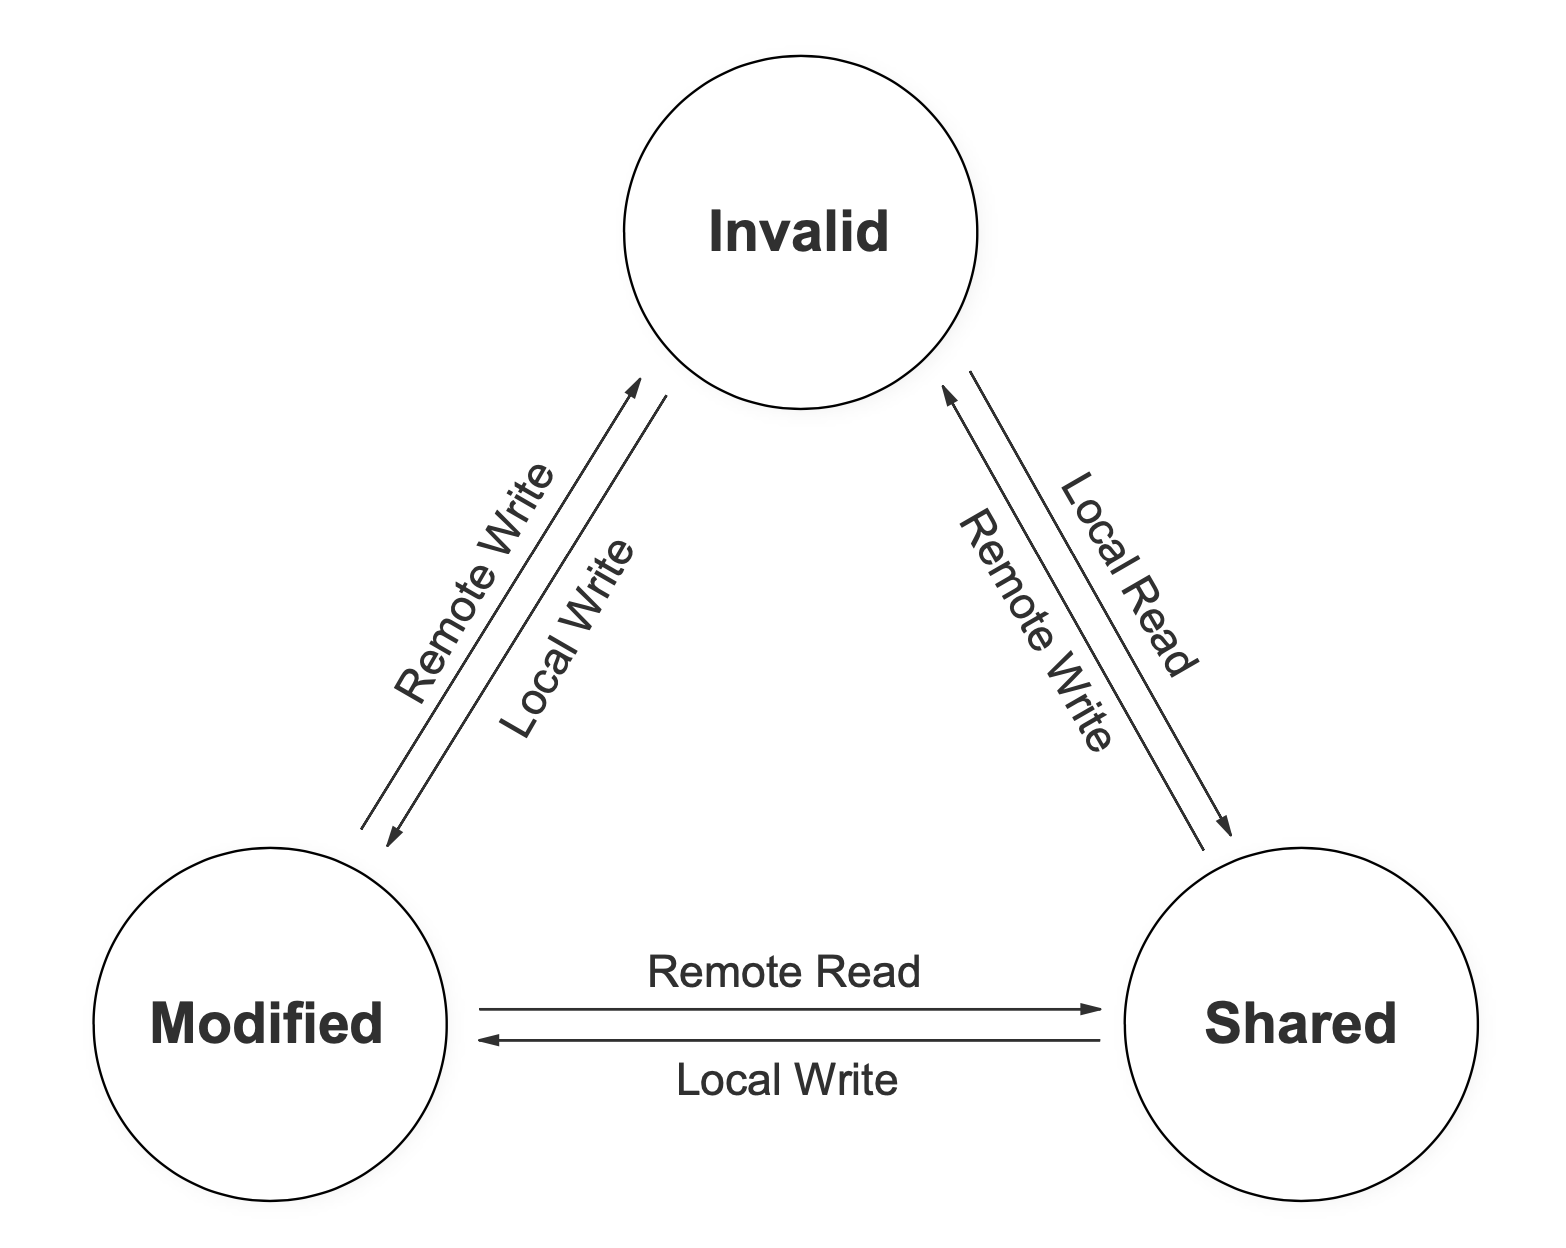
\includegraphics[width=8cm]{msi.png}
      \bicaption[MSI协议状态转化图]
        {MSI协议状态转化图\cite{tcbbd}}
        {Transition of States in MSI protocol}
      \label{fig:MSI}
    \end{figure}
    
    分布式共享内存的主要实现原理是,维护EPT中页表项的状态,即维护虚拟机所拥有物理内存页的状态。如图\ref{fig:MSI},DSM的设计基于Ivy\cite{ivy},Ivy实现了MSI protocol,满足了SC(sequential consistency,顺序一致性)。每个客户机物理页的状态分为Modified:本地vCPU对页作出修改,远程vCPU尚未获得该页的修改,Shared:本地vCPU和远程多个vCPU共享该页,Invalid:需要向其他节点获取该页的最新拷贝,否则本地vCPU无权对该页进行读写。所以,当本地的vCPU发生Page fault时,需要使用RDMA协议或TCP协议向远程节点请求最新的数据页。由于巨型虚拟机中的分布式共享内存需要至少实现x86-TSO(Total Store Order)\cite{tso}弱的内存模型,故节点间内存同步的次数和较弱的内存一致性模型相比更多。如果巨型虚拟机的两个节点上的进程相互共享过多的内存,势必会增加内存同步的开销。分析并减小这类开销是本文关注的重点之一。
    
    \item[I / O虚拟化] I/O虚拟化需要解决的问题有,虚拟机vCPU如何对远程节点上的的模拟设备进行I/O访问,以及如何使得远程的虚拟设备产生的中断准确的路由到对应的vCPU。对于第二个问题,分布式vCPU的虚拟化中对于IPI的处理已经给出了答案,即在QEMU 0上放置master IOAPIC,而在QEMU 1-3上放置dummy IOAPIC。在设备中断到达之后写入dummy IOAPIC时,将信息同步至master IOAPIC,由master IOAPIC将中断通过dummy APIC转发给目的vCPU。对于第一个问题,CPU对设备进行I/O访问有两种方式:PIO(Programmed I/O,针对于x86架构)和MMIO(Memory Mapped I/O)。客户机执行I/O指令后退出到VMM,VMM检查I/O指令的目的设备。如果I/O访问的目的设备是远程机器上的设备,则需要将该请求转发给远程设备,在处理完成后将处理结果发送回来。目前,巨型虚拟机的模拟设备全部放置在master node上。
\end{description}

\section{分布式共享内存性能问题}
综上所述,巨型虚拟机相比于普通虚拟机的实现增加的部分有:(1)分布式共享内存,这一部分需要通过RDMA、TCP等网络协议在集群之间同步物理页的状态;(2)转发机制,将对于远程资源的访问请求转发到对应的节点上去,由真实的资源拥有者处理访问请求。这两部分均会产生网络开销,而网络开销最大的则是分布式共享内存这一组件。由于顺序一致性是是较强的一致性模型,分布式共享内存会产生false sharing(伪共享)现象和page thrashing(页面颠簸)现象\cite{sharing}。伪共享现象是指两个运行在不同CPU核心上的线程不断的写入同一个cache line(缓存行)中的变量,当其中一个线程对变量写入后,另一个核上的缓存行即会失效,于是另一个线程需要从内存中读取最新的数据,而写入变量的线程也需要将缓存行写回主存。如此循环往复即出现了伪共享现象。而页面颠簸现象是由于内存页的换入换出。虚拟内存作为磁盘空间的缓存,可以支持大于物理地址空间的虚拟地址空间。当一个进程频繁访问的页面数量多于总的物理页面数量,或者操作系统为进程选取的驻留集(又称工作集,Resident Set Size, RSS,可以通过ps aux等命令行工具观察进程的驻留集)小于其频繁访问的虚拟空间大小,则会有虚拟页面不断换出到磁盘上,即产生了页面抖动现象。

伪共享现象和页面抖动现象都是因为不同层次的存储器访问延迟大不相同造成的。现代计算机有如下几个存储器层次\cite{csapp}:
\begin{itemize}
  \item L0 寄存器(Register):在CPU内部用来存储指令和数据。通常在一个时钟周期内即可读写数据,用于缓存来自高速缓存(L1-L3)的数据
  \item L1-L3 高速缓存(SRAM):静态RAM(Static Random Access Memory),L1访问需要几个时钟周期(约为4个时钟周期),L2访问需要几十个时钟周期(约为10个时钟周期),L3访问需要近百个时钟周期(约为40个)。L1分为数据缓存(dcache)和指令缓存(icache),L1、L2由单个CPU核独享,L3(LLC, Last Level Cache)由处理器中所有的核共享,保存来自于L4的数据\footnote{数据来源:https://v2ex.com/t/523069}。
  \item L4 主存(DRAM):动态RAM(Dynamic Random Access Memory),访问需要几百个时钟周期(100ns),用来缓存来自磁盘的数据。
  \item L5 本地的二级存储,即磁盘(Disk):磁盘分为SSD(固态硬盘)和HDD(机械硬盘)。SSD一次读取时间为16,000纳秒,HDD一次读取时间为2,000,000纳秒。
  \item L6 远程二级存储(Web服务器等):经过网络协议与网络进行数据交换,访问时间约为150,000,000纳秒。\footnote{数据来源:https://stackoverflow.com/questions/4087280/approximate-cost-to-access-various-caches-and-main-memory}
\end{itemize}

为了获得更大的容量,则会产生更高的延迟。由于分布式共享内存增加了物理内存的容量,需要通过网络访问远程节点的内存,虽然减小了所以引起了更加严重的性能问题。如果在不同节点上的应用程序频繁访问共享的地址空间,则需要分布式共享内存模块进行大量的内存同步工作,不仅造成内存访问的延迟明显提高,使得巨型虚拟机可扩展性降低,还会占用集群中宝贵的网络带宽。虽然分布式共享内存模块已经利用RDMA、压缩优化等技术大大减小了其占用的网络带宽,但仍需要解决根本问题,即对巨型虚拟机的客户机调度器进行重新设计,使得节点间访问共享内存的机会更少,增强客户机内存访问的局部性。
\section{DSM原理介绍}



